\begin{frame}[fragile]{Knowledge Graphs: Entities, Relations, Triples}
  \begin{columns}[T,onlytextwidth]
    \column{0.50\textwidth}
      \begin{itemize}\footnotesize\itemsep0.3em
        \item[\textcolor{red}{$\blacktriangleright$}] \textbf{Knowledge graph (KG):} triples $(h, r, t)$ of head entity, relation and tail entity, $\mathcal{G} \subseteq \mathcal{E} \times \mathcal{R} \times \mathcal{E}$ ($\mathcal{E}$: entities, $\mathcal{R}$: relation types). An \textbf{entity} is a node for one real thing; a \textbf{relation}, a typed, directed edge.
        \item[\textcolor{red}{$\blacktriangleright$}] \textbf{Schema (ontology):} which entity and relation types exist and which types each relation may join; when enforced, it rejects facts that do not fit.
        \item[\textcolor{red}{$\blacktriangleright$}] \textbf{RDF} (Resource Description Framework, a web standard): (subject, predicate, object) triples named by IRIs, web-wide identifiers; an object can also be a literal, such as a date. \textbf{SPARQL} matches graph patterns and aggregates.
        \item[\textcolor{red}{$\blacktriangleright$}] \textbf{Property graph} (e.g.\ Neo4j): labelled nodes, typed directed relationships, key-value properties on both; \textbf{Cypher} queries it.
        \item[\textcolor{red}{$\blacktriangleright$}] \textbf{Scale:} Wikidata had more than 120 million items on 6 Oct.\ 2026. CypherBench, a text-to-Cypher benchmark, counts over 4 million entity types and 12{,}000 relation types in Wikidata's schema: far too many for a prompt.
      \end{itemize}
    \column{0.48\textwidth}
      \centering
      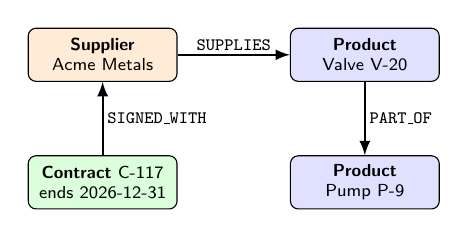
\begin{tikzpicture}[font=\sffamily\scriptsize, >=latex, scale=0.9,
          every node/.style={transform shape},
          ent/.style={draw, rounded corners=0.1cm, align=center, minimum width=2.1cm, minimum height=0.75cm},
          sup/.style={ent, fill=orange!16},
          prod/.style={ent, fill=blue!12},
          con/.style={ent, fill=green!14},
          rel/.style={->, thick},
          rtag/.style={font=\ttfamily\scriptsize, inner sep=1.5pt}]
        \node[sup]  (s) at (0,2.0)   {\textbf{Supplier}\\Acme Metals};
        \node[prod] (v) at (3.7,2.0) {\textbf{Product}\\Valve V-20};
        \node[prod] (p) at (3.7,0.2) {\textbf{Product}\\Pump P-9};
        \node[con]  (c) at (0,0.2)   {\textbf{Contract} C-117\\ends 2026-12-31};
        \draw[rel] (s) -- node[rtag, above] {SUPPLIES} (v);
        \draw[rel] (v) -- node[rtag, right] {PART\_OF} (p);
        \draw[rel] (c) -- node[rtag, right] {SIGNED\_WITH} (s);
      \end{tikzpicture}\\[0.2em]
\begin{lstlisting}[basicstyle=\ttfamily\scriptsize, showstringspaces=false, frame=single, rulecolor=\color{gray!60}]
MATCH (s:Supplier)-[:SUPPLIES]->(:Product)
        -[:PART_OF]->(:Product {name: 'Pump P-9'}),
      (c:Contract)-[:SIGNED_WITH]->(s)
WHERE c.ends < date('2027-01-01')
RETURN s.name, c.id
\end{lstlisting}
      {\scriptsize Which suppliers of parts of pump P-9 hold a contract that ends before 2027? The query returns Acme Metals, C-117.\par}
      \vspace{0.2em}
      {\scriptsize Pan et al., IEEE TKDE 2024; W3C, \href{https://www.w3.org/TR/rdf11-concepts/}{RDF 1.1}, \href{https://www.w3.org/TR/sparql11-query/}{SPARQL 1.1}; \href{https://neo4j.com/docs/getting-started/appendix/graphdb-concepts/}{Neo4j docs}; \href{https://www.wikidata.org/wiki/Wikidata:Statistics}{Wikidata statistics}; Feng et al., ACL 2025.\par}
  \end{columns}
\end{frame}

\begin{frame}{Building a Knowledge Graph With an LLM}
  \begin{columns}[T,onlytextwidth]
    \column{0.52\textwidth}
      \begin{itemize}\footnotesize\itemsep0.3em
        \item[\textcolor{red}{$\blacktriangleright$}] \textbf{Roadmap} (Pan et al.): ``KG-enhanced LLMs'' (the graph feeds the model), ``LLM-augmented KGs'' (the model works on the graph, e.g.\ builds or completes it), and ``Synergized LLMs + KGs'' (each improves the other). Building a graph is the second; retrieving from it, the first.
        \item[\textcolor{red}{$\blacktriangleright$}] \textbf{Extraction:} per chunk, an LLM lists entities and relations of the schema's types; structured outputs keep it parseable. \textbf{Coreference resolution} maps ``the chipmaker'' to NeoChip.
        \item[\textcolor{red}{$\blacktriangleright$}] \textbf{Entity resolution:} merging the names of one real entity (``NC'', ``NeoChip'') into one node. GraphRAG matches exact strings; HippoRAG links names whose embeddings have cosine similarity above 0.8.
        \item[\textcolor{red}{$\blacktriangleright$}] \textbf{Quality:} relations ``may not be explicitly stated in the text'' (GraphRAG). Recall drops with length: GPT-4 found almost twice as many entity references in 600- as in 2{,}400-token chunks; HippoRAG's extraction F1 falls from 71.8 (10 shortest passages) to 53.9 (10 longest). Keep each triple's source.
      \end{itemize}
    \column{0.46\textwidth}
      \centering
      \resizebox{\linewidth}{!}{%
      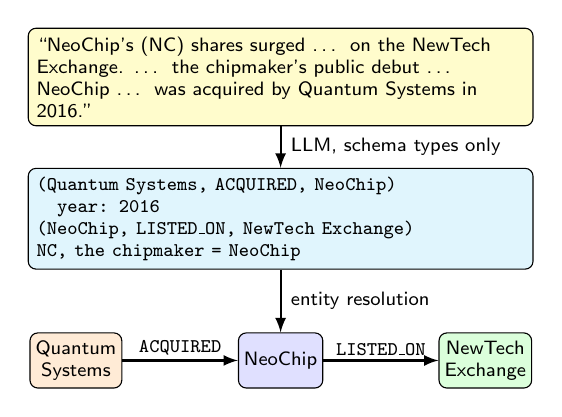
\begin{tikzpicture}[font=\sffamily\scriptsize, >=latex,
          txt/.style={draw, rounded corners=0.1cm, align=left, text width=6.2cm, inner sep=3pt},
          ent/.style={draw, rounded corners=0.1cm, align=center, minimum height=0.7cm, inner sep=2pt},
          rel/.style={->, thick},
          rtag/.style={font=\ttfamily\scriptsize, inner sep=1.5pt}]
        \node[txt, fill=yellow!20] (chunk) at (0,3.0) {``NeoChip's (NC) shares surged \ldots{} on the NewTech Exchange. \ldots{} the chipmaker's public debut \ldots{} NeoChip \ldots{} was acquired by Quantum Systems in 2016.''};
        \node[txt, fill=cyan!12, font=\ttfamily\scriptsize] (trip) at (0,1.2) {(Quantum Systems, ACQUIRED, NeoChip)\\\quad year: 2016\\(NeoChip, LISTED\_ON, NewTech Exchange)\\NC, the chipmaker = NeoChip};
        \node[ent, fill=orange!16] (q) at (-2.6,-0.6) {Quantum\\Systems};
        \node[ent, fill=blue!12]   (n) at (0,-0.6)    {NeoChip};
        \node[ent, fill=green!14]  (x) at (2.6,-0.6)  {NewTech\\Exchange};
        \draw[rel] (chunk) -- node[right] {LLM, schema types only} (trip);
        \draw[rel] (trip) -- node[right] {entity resolution} (n);
        \draw[rel] (q) -- node[rtag, above] {ACQUIRED} (n);
        \draw[rel] (n) -- node[rtag, above] {LISTED\_ON} (x);
      \end{tikzpicture}}\\[0.3em]
      {\scriptsize Passage from GraphRAG's extraction example (Edge et al., \href{https://arxiv.org/abs/2404.16130v2}{arXiv:2404.16130v2}, Sec.~3.1.2; matching and quote: Sec.~3.1.3; chunk sizes: App.~A.2); triples and merges drawn for this slide. Pan et al., ``Unifying Large Language Models and Knowledge Graphs: A Roadmap,'' IEEE TKDE 2024, \href{https://arxiv.org/abs/2306.08302v3}{arXiv:2306.08302v3}, Sec.~3.1; Guti\'errez et al., \href{https://arxiv.org/abs/2405.14831v3}{arXiv:2405.14831v3}, Sec.~3.4 and Table~16.\par}
  \end{columns}
\end{frame}

\begin{frame}{GraphRAG for Corpus-Wide Questions}
  \begin{columns}[T,onlytextwidth]
    \column{0.56\textwidth}
      \begin{itemize}\footnotesize\itemsep0.3em
        \item[\textcolor{red}{$\blacktriangleright$}] \textbf{Global questions} (``What are the main themes in the dataset?'') cover the whole corpus; top-$k$ retrieval sees only a sample of it.
        \item[\textcolor{red}{$\blacktriangleright$}] \textbf{Index:} an LLM extracts entities, relationships and claims from every 600-token chunk; a 1M-token podcast corpus gave 8{,}564 nodes and 20{,}691 edges.
        \item[\textcolor{red}{$\blacktriangleright$}] \textbf{Communities:} community detection splits a graph into densely connected groups. GraphRAG runs \textbf{Leiden} recursively, which maximizes modularity (edges inside groups above the number expected by chance) and keeps every group connected. The LLM summarizes every community at each level, C0 (root) to C3.
        \item[\textcolor{red}{$\blacktriangleright$}] \textbf{Answer:} map summary batches to partial answers scored 0--100 for helpfulness; reduce the best to one.
        \item[\textcolor{red}{$\blacktriangleright$}] \textbf{Result:} an LLM judge preferred GraphRAG to vector RAG in 72--79\% of comprehensiveness and 62--81\% of diversity comparisons (125 questions per corpus); vector RAG stayed the most direct. Root summaries need over 97\% fewer tokens than summarizing the raw text.
      \end{itemize}
    \column{0.42\textwidth}
      \centering
      \vspace{0.3em}
      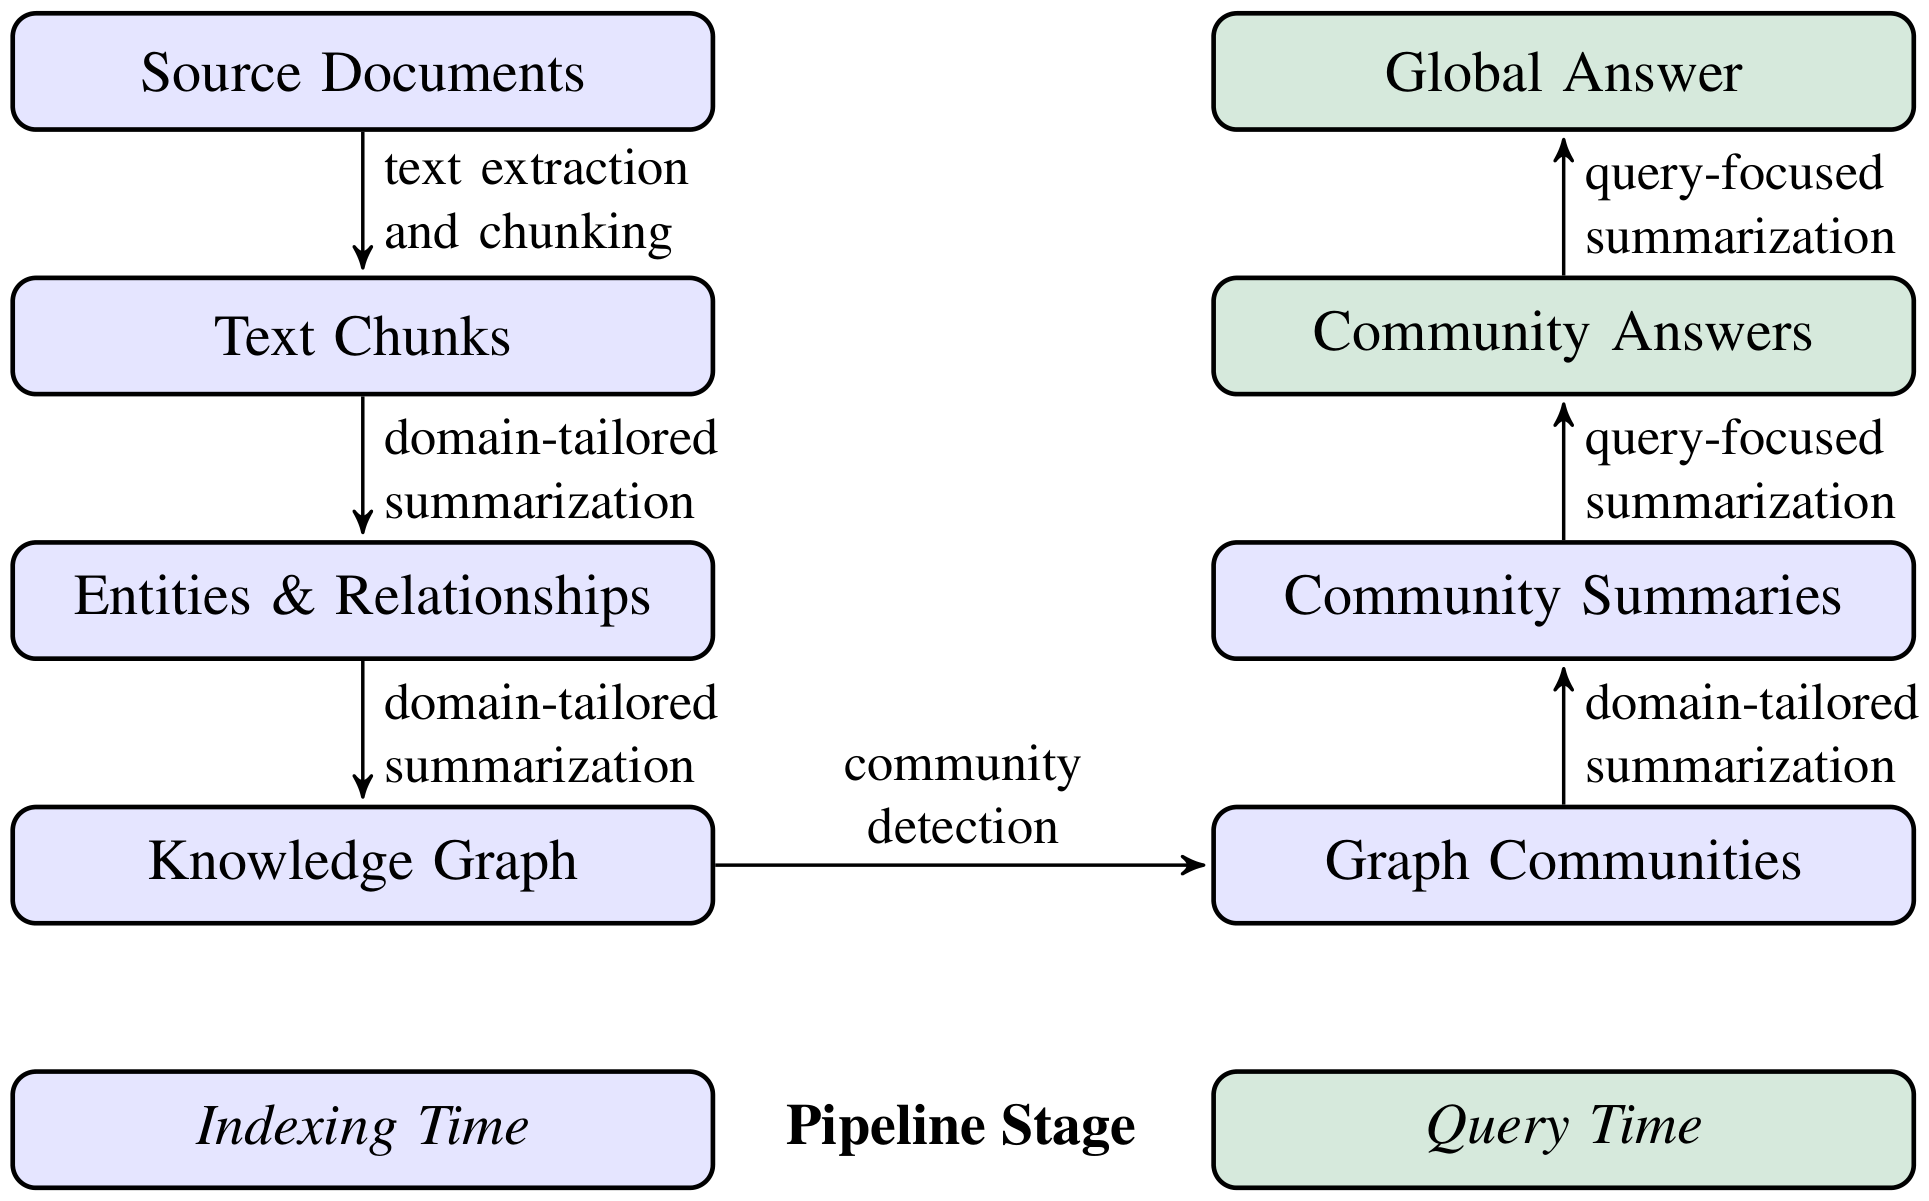
\includegraphics[width=\linewidth,height=0.56\textheight,keepaspectratio]{images/nlp-security-enterprise/graphrag_fig1_pipeline.png}\\[0.2em]
      {\scriptsize Edge et al., ``From Local to Global: A Graph RAG Approach to Query-Focused Summarization,'' \href{https://arxiv.org/abs/2404.16130v2}{arXiv:2404.16130v2}, Figure~1 (results: Figure~2). Leiden: Traag et al., \emph{Scientific Reports} 2019, \href{https://arxiv.org/abs/1810.08473v3}{arXiv:1810.08473v3}.\par}
  \end{columns}
\end{frame}

\begin{frame}{HippoRAG: Multi-Hop Retrieval With PageRank}
  \begin{columns}[T,onlytextwidth]
    \column{0.52\textwidth}
      \begin{itemize}\footnotesize\itemsep0.3em
        \item[\textcolor{red}{$\blacktriangleright$}] \textbf{Multi-hop:} ``Which Stanford professor works on the neuroscience of Alzheimer's?'' joins passages that never mention each other.
        \item[\textcolor{red}{$\blacktriangleright$}] \textbf{Index:} an LLM turns each passage into open triples, a schemaless KG; an encoder adds synonym edges (MuSiQue: 11{,}656 passages, 91{,}729 nodes).
        \item[\textcolor{red}{$\blacktriangleright$}] \textbf{Query:} the question's entities are linked to KG nodes. \textbf{Personalized PageRank} (PPR) scores each node by the long-run share of time a random walk spends there if it restarts at a query node with probability $\alpha$:
          \[ \mathbf{p} = \alpha\,\mathbf{s} + (1-\alpha)\,W^{\top}\mathbf{p}, \qquad \mathbf{r} = M^{\top}\mathbf{p} \]
          {\scriptsize $W$: row-normalized adjacency; $\mathbf{s}$: restart mass on query nodes, each weighted by $1/$(passages containing it); $\alpha = 0.5$; $\mathbf{p}$: node scores; $M$: node-passage counts; $\mathbf{r}$: passage scores.\par}
        \item[\textcolor{red}{$\blacktriangleright$}] \textbf{Cost} against IRCoT (retrieval interleaved with chain-of-thought steps): online 10--30$\times$ cheaper and 6--13$\times$ faster; QA on par or better on MuSiQue and 2Wiki, 3.4 F1 lower on HotpotQA; indexing about 10$\times$ slower.
      \end{itemize}
    \column{0.46\textwidth}
      \centering
      \vspace{0.6em}
      {\footnotesize
      \begin{tabular}{@{}l r r@{}}
        \toprule
        \textbf{Recall@5 (\%)} & \textbf{MuSiQue} & \textbf{2Wiki} \\
        \midrule
        ColBERTv2 & 49.2 & 68.2 \\
        HippoRAG & 51.9 & 89.1 \\
        \quad without PPR & 41.0 & 61.4 \\
        IRCoT + HippoRAG & 57.6 & 93.9 \\
        \bottomrule
      \end{tabular}\par}
      \vspace{0.4em}
      {\scriptsize Recall@5: share of supporting passages ranked in the top five, on two multi-hop QA sets (2Wiki: 2WikiMultiHopQA). ColBERTv2: a late-interaction retriever.\par}
      \vspace{0.4em}
      {\scriptsize Guti\'errez et al., ``HippoRAG: Neurobiologically Inspired Long-Term Memory for Large Language Models,'' NeurIPS 2024, \href{https://arxiv.org/abs/2405.14831v3}{arXiv:2405.14831v3}, Figure~1, Secs.~2.2--2.3 and~3.4, Tables~1--5, App.~G. PPR: Haveliwala, WWW 2002. IRCoT: Trivedi et al., ACL 2023.\par}
  \end{columns}
\end{frame}

\begin{frame}{Text-to-Query and Choosing a Method}
  \begin{itemize}\footnotesize\itemsep0.3em
    \item[\textcolor{red}{$\blacktriangleright$}] \textbf{Text-to-query:} the LLM writes a Cypher or SPARQL query from the schema; the database runs it, so counts and averages over thousands of entities are exact, with no top-$k$ cut.
    \item[\textcolor{red}{$\blacktriangleright$}] \textbf{Risk:} a valid query for the wrong question gives a confident wrong answer. On CypherBench the best model's results matched the reference query's for 61.58\% of questions.
    \item[\textcolor{red}{$\blacktriangleright$}] \textbf{Controls:} check relation types and directions against the schema before running; use read-only, narrowly scoped credentials; cap the rows; show the query beside the answer.
  \end{itemize}
  \vspace{0.2em}
  {\centering\scriptsize
  \begin{tabular}{>{\raggedright\arraybackslash}p{1.8cm} >{\raggedright\arraybackslash}p{2.8cm} >{\raggedright\arraybackslash}p{4.4cm} >{\raggedright\arraybackslash}p{2.9cm}}
    \toprule
    \textbf{Method} & \textbf{Best for} & \textbf{Indexing cost} & \textbf{Freshness} \\
    \midrule
    Vector RAG & facts stated in one or a few chunks & one embedding per chunk & re-embed the changed chunks \\
    \addlinespace[0.15em]
    GraphRAG & themes and summaries across the corpus & LLM calls per chunk and per community; 281 min (GPT-4-Turbo, 1M tokens) & changed communities need new summaries \\
    \addlinespace[0.15em]
    HippoRAG & multi-hop questions about entities & LLM triple extraction per passage, about 10$\times$ slower than dense indexing & new passages add nodes and edges \\
    \addlinespace[0.15em]
    Text-to-query & counts, aggregates, exact filters & a curated graph and schema; no LLM pass & live: each query reads the database \\
    \bottomrule
  \end{tabular}\par}
  \vspace{0.2em}
  {\scriptsize Feng et al., ``CypherBench: Towards Precise Retrieval over Full-scale Modern Knowledge Graphs in the LLM Era,'' ACL 2025, \href{https://aclanthology.org/2025.acl-long.438/}{aclanthology.org/2025.acl-long.438}, Sec.~6.1; credentials: \texttt{GraphCypherQAChain} security note, \href{https://github.com/langchain-ai/langchain-neo4j}{github.com/langchain-ai/langchain-neo4j}; costs: Edge et al., Guti\'errez et al.\par}
\end{frame}
